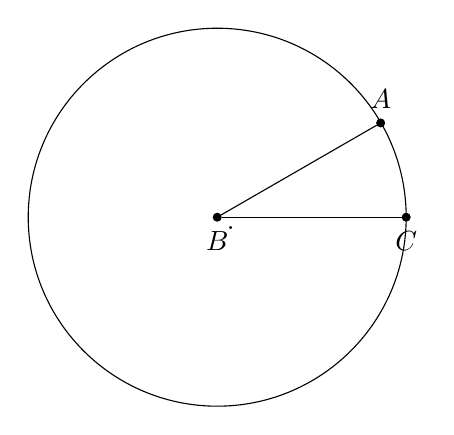
\begin{tikzpicture}
[scale =0.3,>=stealth,point/.style = {draw, circle, fill = black, inner sep = 1pt},]
\node (B) at (0,0)[point,label=below :$B$] {};
\node (C) at (8,0)[point,label=below :$C$] {};
\node (A) at (6.92,3.99)[point,label=above :$A$] {};
\draw (0,0) node [below right] {.} circle (8);
\draw (B)--(A);
\draw (B)--(C);
\end{tikzpicture}

